\documentclass[english]{DESCARWINreport}

\usepackage{amsmath}
\usepackage{amsfonts}
\usepackage{color}
\usepackage{algorithm}
\usepackage[noend]{algorithmic}
%\usepackage{algorithmic}
\usepackage{subfigure}
\usepackage{hyperref}
\hypersetup{colorlinks=true,linkcolor=black}
\usepackage{lscape}
\title{DESCARWIN\\\bigskip {\em \LARGE The Marriage of Descartes and Darwin}\\\vspace{8cm} 
{\LARGE D3.3\\
Multi-objective Experimentations}}
%ANR-09-COSI-002
%\author{Pierre Savéant and Johann Dréo}
\date{\today}
\laboratory{TRT - INRIA - ONERA}
\docref{62 441 217-306}
\revision{-}

\setlength{\parindent}{0cm}
\setlength{\parskip}{2ex plus 0.5ex minus 0.2ex}

\newcounter{hyp}
\setcounter{hyp}{1}
\newcommand{\hyp}{H\thehyp\stepcounter{hyp}}
\newcounter{defi}
\setcounter{defi}{1}
\newcommand{\defi}{D\thedefi\stepcounter{defi}}
\newcounter{con}
\setcounter{con}{1}
\newcommand{\con}{C\thecon\stepcounter{con}}

% Pour réduire globalement l'espace entre les items d'une liste
% on peut également utiliser le bout de code suivant de M. Wooding
% Les paramètres utilisés pour définir cette mise en page
% sont les suivants :
% \topsep espace vertical supplémentaire (ajoute à \parskip)
% 	inséré entre le texte précédant la liste et le 1er objet
% 	de la liste
% \partosep espace vertical supplémentaire inséré devant la liste
% 	si celle-ci est précédée d'une ligne blanche
% \itemsep espace vertical supplémentaire (ajouté à \parsep)
% 	inséré entre les éléments d'une liste.

%%%% debut macro %%%%
\makeatletter
\toks@\expandafter{\@listI}
% \edef\@listI{\the\toks@\setlength{\parsep}{0pt}}
% \edef\@listI{\the\toks@\setlength{\topsep}{0pt}}
\makeatother
%%%% fin macro %%%%

\usepackage[final]{pdfpages}

\hoffset -2cm
\textwidth 15cm

\newcommand{\DAE}{{\sc DaE}}
\newcommand{\DAEYAHSP}{{\sc DaE$_{\text{YAHSP}}$}}

\begin{document}

\maketitle

%\cleardoublepage

\begin{revisions}
\begin{revtable}
\dates{May 7., 2013}{}{}{}{}
\writers{Johann Dr\'eo\\Mostepha Khouadjia\\Pierre Savéant\\Marc Schoenauer\\Vincent Vidal}{}{}{}
\approvers{P. Sav\'eant}{}{}{}
\end{revtable}
\begin{revisionlabels}
\revlabel{initial version}
\revlabel{}
\end{revisionlabels}
\end{revisions}

%\begin{figure}[htbp]
%\vspace{-0.5cm}
%\centering
%\includegraphics[width=0.25\textwidth]{Salon_du_Bourget_20090619_114_GroundSearch_1000km.jpg}
%\end{figure}

\begin{abstract}
The object of this document is to provide results of the experimentation campaign regarding the original multi-objective approach to AI planning developed in the Descarwin project. It is made of 3 chapters, corresponding to 3 publications describing the different steps of the experimental campaign that validates our approach to Pareto-based multi-objective AI planning. Each chapter starts with an extended abstract that introduces the context of the work, followed by a copy of the published paper.

Note that all experiments that are described in this deliverable include an intensive parameter tuning phase before any result is reported. The detailed procedure uses the ParamILS framework, as described in deliverable 2.3.

\begin{itemize}
 \item The first validation was performed on the original {\tt Zeno} benchmark suite, as described in Deliverable 3.1. The benchmark is first described in detail, and the experimental parts compare several multi-objective evolutionary engines in several instances of this benchmark. And the winner is (on the Zeno testbench at least) \ldots the Indicator-Based Evolutionary Algorithm (IBEA) that uses as indicator the hypervolume. Hence only $IBEA_{Hv}$ has been considered in all following experiments.

This work has been published as: ``Mostepha Redouane Khouadjia, Marc Schoenauer, Vincent Vidal, Johann Dréo and Pierre Savéant, {\em Multi-Objective AI Planning: Evaluating DaEYAHSP on a Tunable Benchmark}. In Robin C. Purshouse, Peter J. Fleming, and Carlos M. Fonseca, Eds, Proc. 7th International Conference on Evolutionary Multi-Criterion Optimization (EMO2013), pp 36-50, LNCS 7811, Springer Verlag, 2013.'' 

\item The second validation compares the Pareto-based approach that was found the best-performing in the previous chapter, i.e. $IBEA_{Hv}$, with the more traditional aggregation-based approach using the single objective version of \DAE. An intersting issue is that of the measure to use within ParamILS, the off-line parameter tuning procedure, for the aggregated approach: the discussion about this issue is reported in Deliverable 2.3, and was surprising enough to be published in the LION'7 conference, and hence will not be detailed in this delivrable. The results presented here all use the hypervolume indicator as a measure of goodness for the tuning of the aggregated single-objective runs. The testbench is, again, the {\tt Zeno} benchmark, and most results demonstrate the superiority of the Pareto-based multi-objective approach compared to the aggregated approach, both in terms of quality of the solution and in terms of speed.

This work has been published as: ``Mostepha Redouane Khouadjia, Marc Schoenauer, Vincent Vidal, Johann Dréo and Pierre Savéant, {\em Multi-Objective AI Planning: Comparing Aggregation and Pareto Approaches}. In Martin Middendorf and Christian Blum, Eds, Proc. 13th European Conference on Evolutionary Computation in Combinatorial Optimisation (EvoCOP2013), pp 202-213, LNCS 7832, Springer Verlag, 2013.''

\item The last series of experiments validates the multi-objective \DAEYAHSP\ approach against the only competitor from the AI Planning community, i.e. the approach using the metric-sensitive planner LPG, one of the state-of-the-art planner in single-objective setting, that can however directly handle aggregated objectives. The comparative experiments here involve not only the {\tt Zeno} test-bench, but also the other domains and instances proposed in Deliverable 3.1 based on the multi-objectivizations of some IPC7 (single-objective) domains. In most cases, \DAEYAHSP\ is found to outperform the LPG-based approach.

This work has been accepted at IJCAI 2013 conference, August 2013, as ``Mostepha Redouane Khouadjia, Marc Schoenauer, Vincent Vidal, Johann Dréo and Pierre Savéant, {\em Pareto-Based Multiobjective AI Planning}. In Proc. 23rd International Joint Conference on Artificial Intelligence (IJCAI 2013), 2013.''
\end{itemize}



\end{abstract}

%\begin{figure}[htbp]
%\centering
%\includegraphics[width=0.70\textwidth]{../Images/Salon_du_Bourget_20090619_114_GroundSearch_1000km.jpg}
%\end{figure}

\tableofcontents

\newpage

\chapter{Evaluating \DAEYAHSP\ on a Tunable Benchmark}



\newpage
\hoffset 0cm
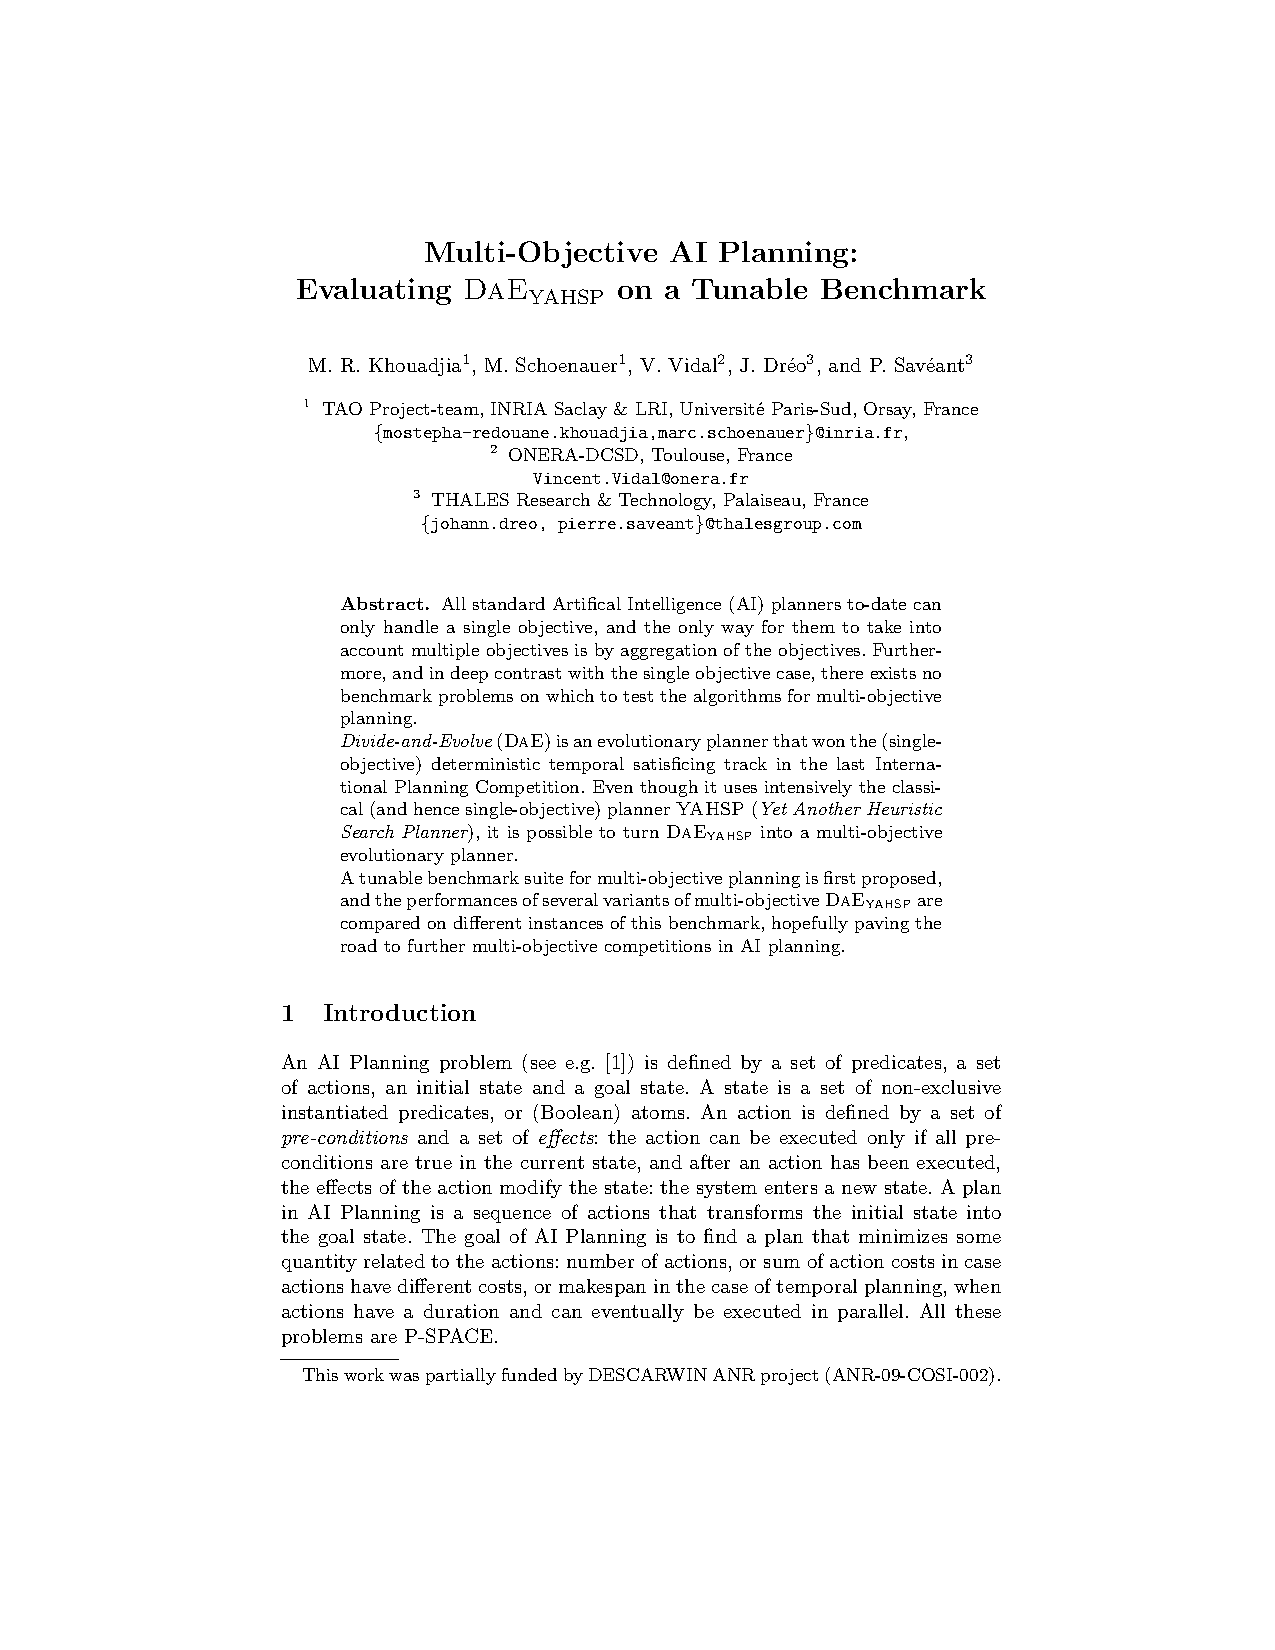
\includepdf[height=32cm,pages=-,offset=0cm -4cm]{emo2012.pdf}
\newpage
\hoffset -2cm

\chapter{Comparing Aggregation and Pareto Approaches}

\newpage
\hoffset 0cm
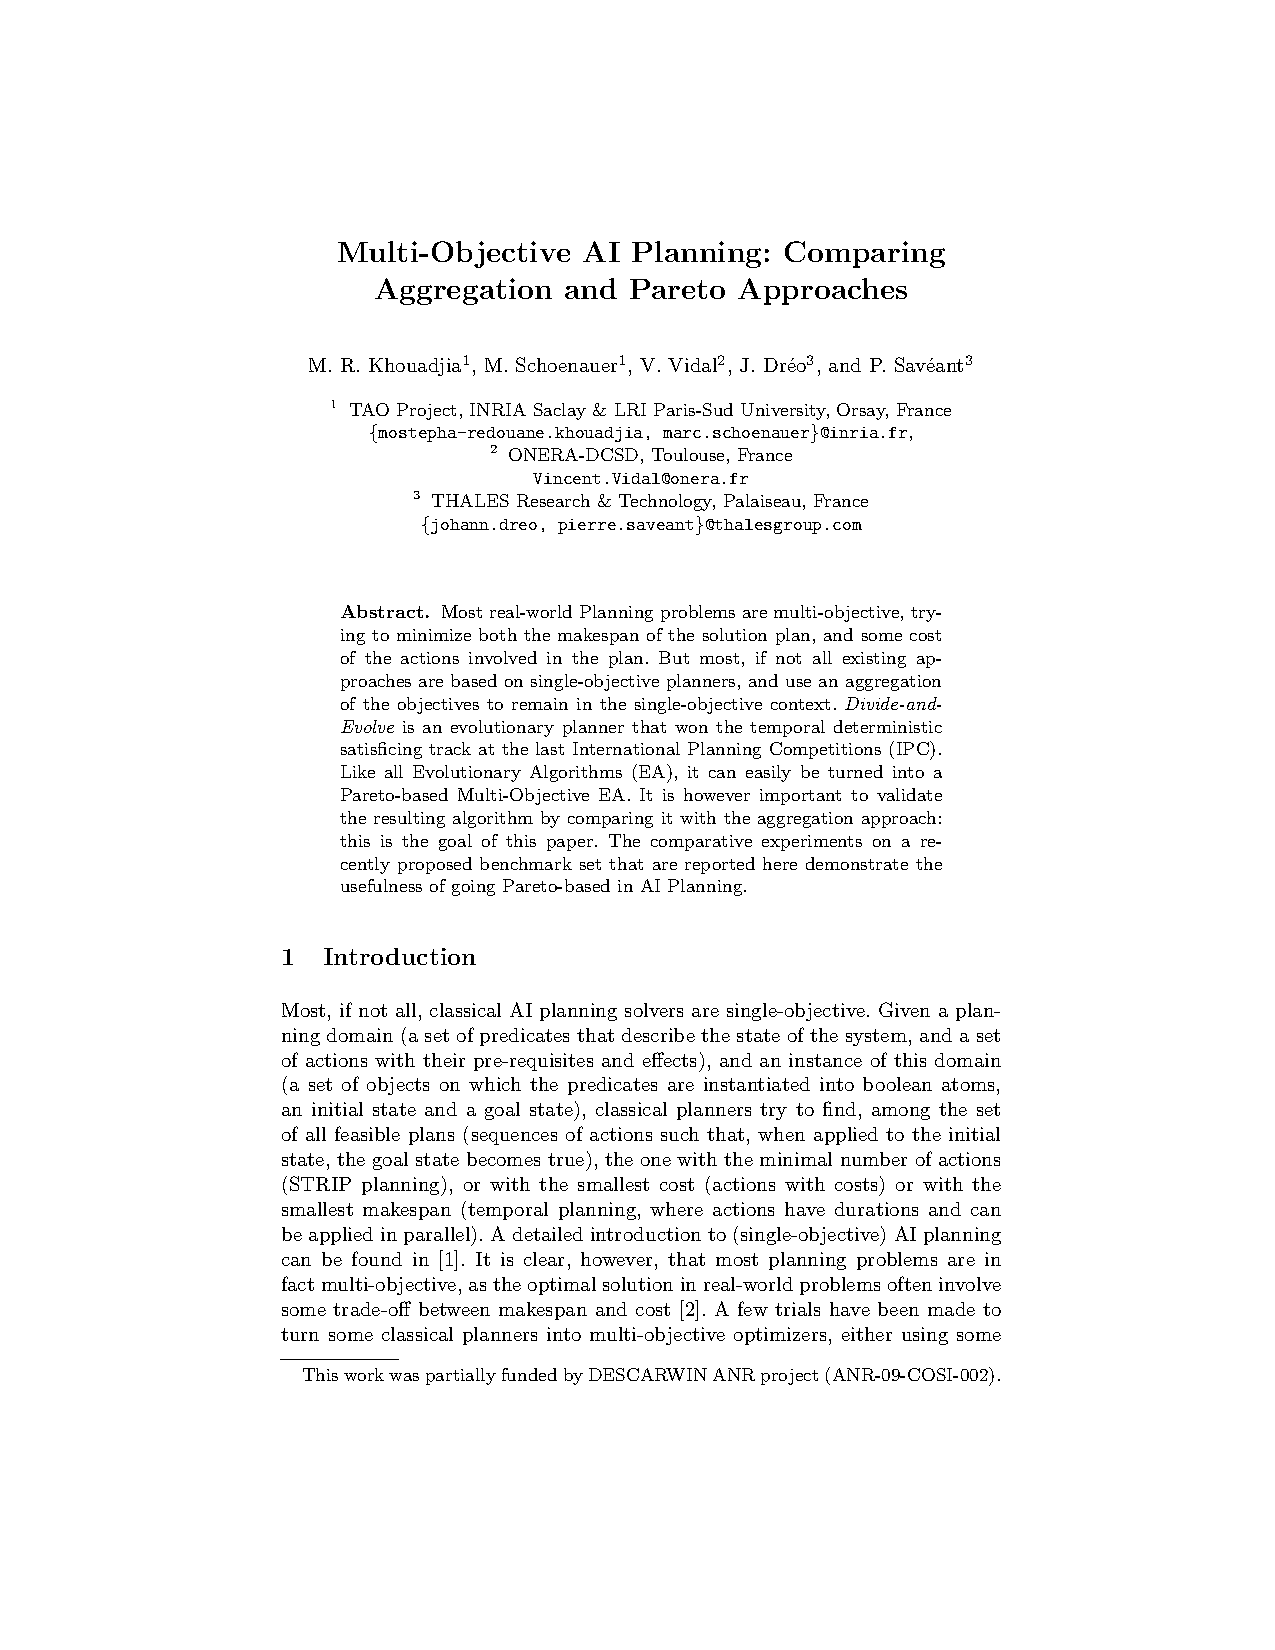
\includepdf[height=32cm,pages=-,offset=0cm -4cm]{evocop2012.pdf}
\newpage
\hoffset -2cm

\chapter{Comparing Metric-Sensitive and Pareto Approaches}

\newpage
\hoffset 0cm
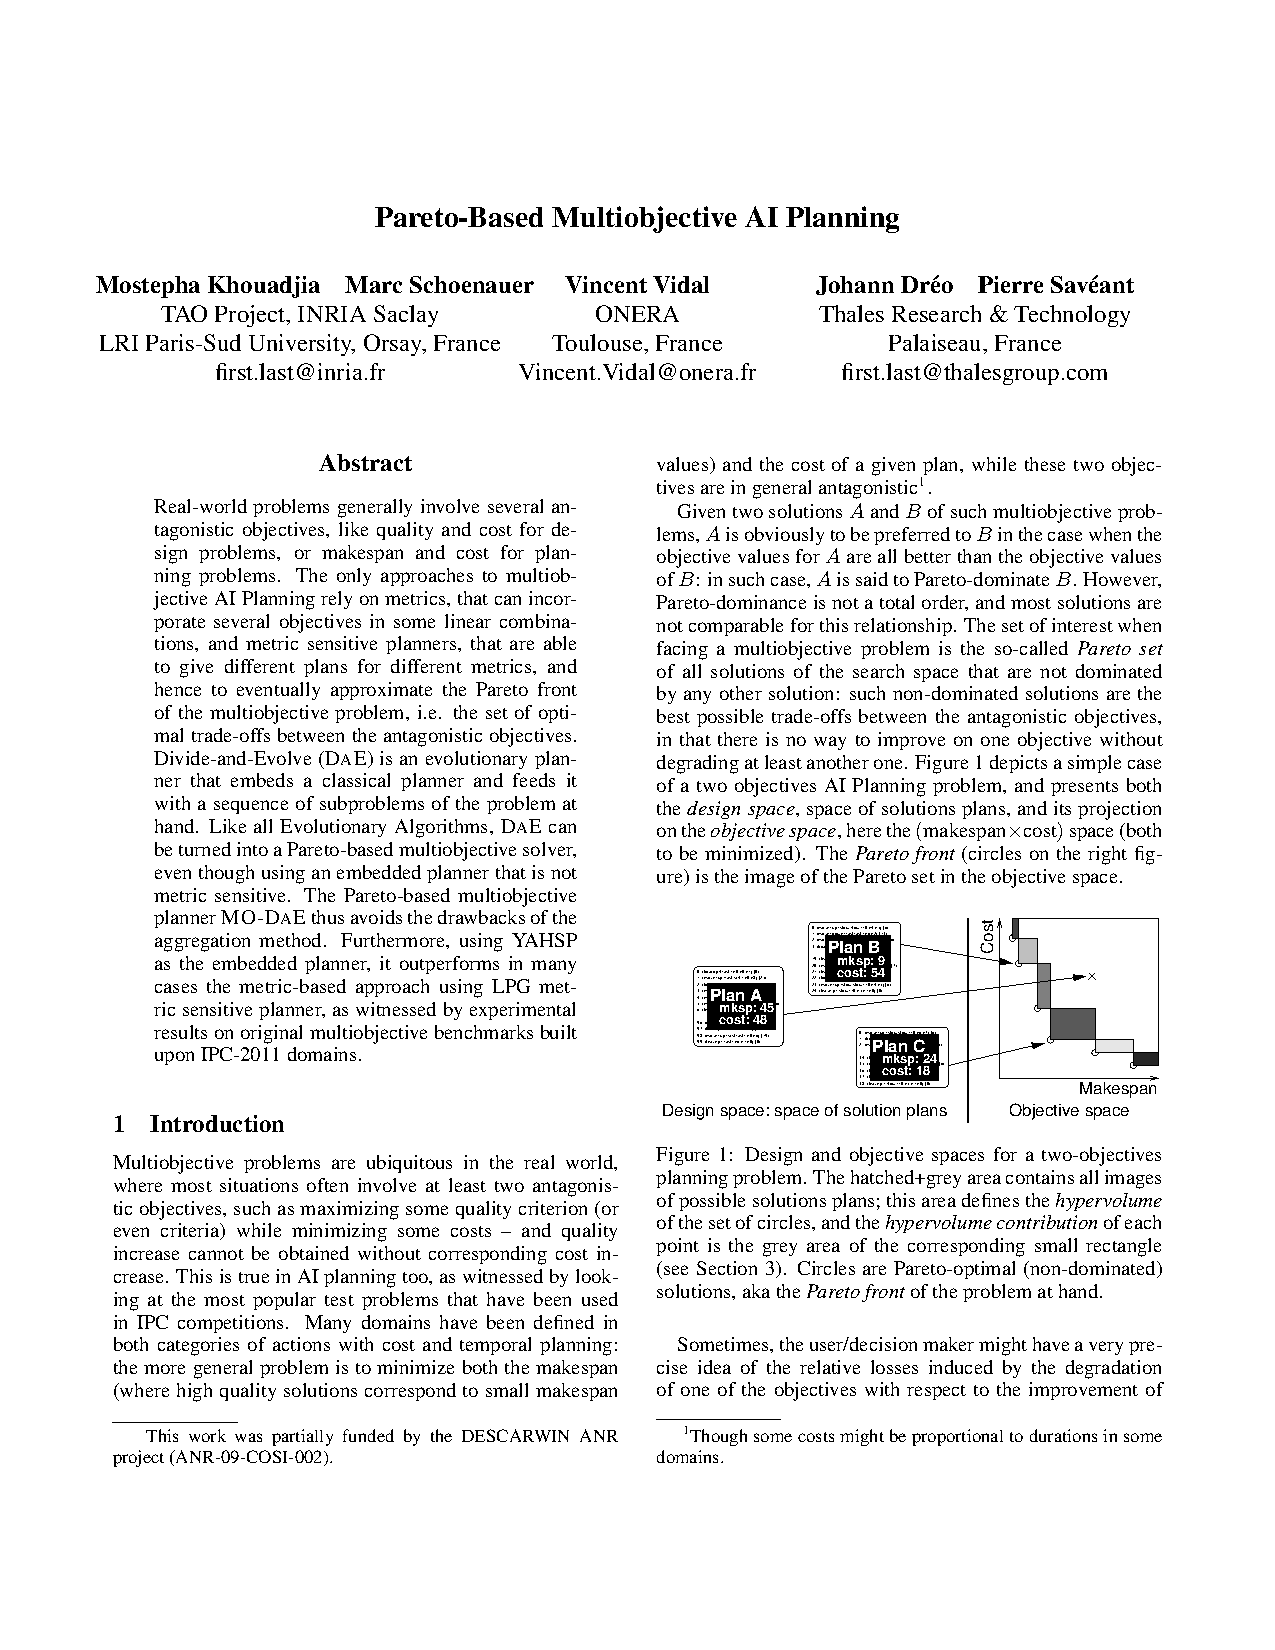
\includepdf[width=22.5cm,height=32cm,pages=-,offset=0cm -4cm]{567.pdf}
\hoffset -2cm


\end{document}